\documentclass[10pt,twocolumn,letterpaper]{article}
\usepackage{wacv,times,epsfig,graphicx,amsmath,amssymb}
\usepackage{caption,subcaption,multirow,bigstrut,paralist}


\usepackage[pagebackref=true,breaklinks=true,letterpaper=true,colorlinks,bookmarks=false]{hyperref}

\newcommand{\todo}[1]{\textcolor{red}{todo: {\em #1}}}
\newcommand{\figref}[1]{Figure~\ref{fig:#1}}
\newcommand{\tblref}[1]{Table~\ref{tbl:#1}}

%\wacvfinalcopy % *** Uncomment this line for the final submission

\def\wacvPaperID{****} % *** Enter the wacv Paper ID here
\def\httilde{\mbox{\tt\raisebox{-.5ex}{\symbol{126}}}}

% Pages are numbered in submission mode, and unnumbered in camera-ready
\ifwacvfinal\pagestyle{empty}\fi
\setcounter{page}{1}


\begin{document}


%\title{Deep Methods for Estimating Transient Scene Properties}
\title{A Fast Method for Estimating Transient Scene Properties}


\author{Ryan Baltenberger, Connor Greenwell, Scott Workman, Nathan Jacobs \\
  \vspace{-.75em} 
  Department of Computer Science, University of Kentucky \\
  {\tt\small \{rbalten, connor, scott, jacobs\}@cs.uky.edu}
}

\maketitle
\ifwacvfinal\thispagestyle{empty}\fi


\begin{abstract}

We propose to use deep convolutional neural networks to estimate the
transient attributes of a scene from a single image.  Transient scene
attributes describe both the objective conditions, such as the
weather, time of day, and the season, and subjective properties of a
scene, such as whether or not the scene seems busy. Recently,
convolutional neural networks have been used to achieve
state-of-the-art results for many vision problems, from object
detection to scene classification, but have not previously been used
for estimating transient attributes. We compare several methods for
adapting an existing network architecture and present state-of-the-art
results on two benchmark datasets. Our method is more accurate and
significantly faster than all previous methods, enabling real-world
applications. 

\end{abstract}

\section{Introduction}
% general intro to the problem and why it is important
Outdoor scenes experience a wide range of lighting and weather conditions which
dramatically affect their appearance. A scene can change from rainy and
brooding to sunny and pleasant in a matter of hours, even minutes. The ability
to quickly understand these fleeting, or transient, attributes is a critical
skill that people often take for granted. Automatically understanding such
subtle conditions has many potential applications, including: improving
context-dependent anomaly detection~\cite{abrams12lost}; enabling
attribute-oriented browsing and search of large image
sets\cite{jacobs07amos,skyfinder}; estimating micro-climate conditions using
outdoor webcams~\cite{islam13webcamweather}; as a pre-processing step for
higher-level algorithms for
calibration~\cite{jacobs13cloudcalibration,workman2014rainbow}, shape
estimation~\cite{heliometric,abramsheliometric},
geolocalization~\cite{jacobs07geolocate}; and  environmental
monitoring~\cite{jacobs09webcamgis}. 

% what do we propose to do? 

We propose a fast method for predicting transient attributes from a single
image using deep convolutional neural networks (CNNs). CNNs have been used to
obtain state-of-the-art results in problems ranging from object
classification~\cite{krizhevsky2012imagenet}, object
detection~\cite{girshick2013rich}, and scene
classification~\cite{zhou2014places} but have not been used to estimate
transient scene attributes. Our work addresses two specific problems related to
estimating transient scene attributes. First, the problem of estimating whether
it is sunny or cloudy~\cite{lutwoclass} and second, predicting the degree to
which various transient attributes are present in the scene~\cite{Laffont14}.
To this end, we present two different networks and three different training
methods. Our methods achieve state-of-the-art results on two benchmark
datasets, despite being significantly faster.  \figref{cartoon} shows an
overview of our method.  Input images are pushed through the specially trained
CNN that outputs a set of attribute values.

%\figref{results} shows the output of our
%methods for several example images.

\begin{figure}[t]
	\centering
		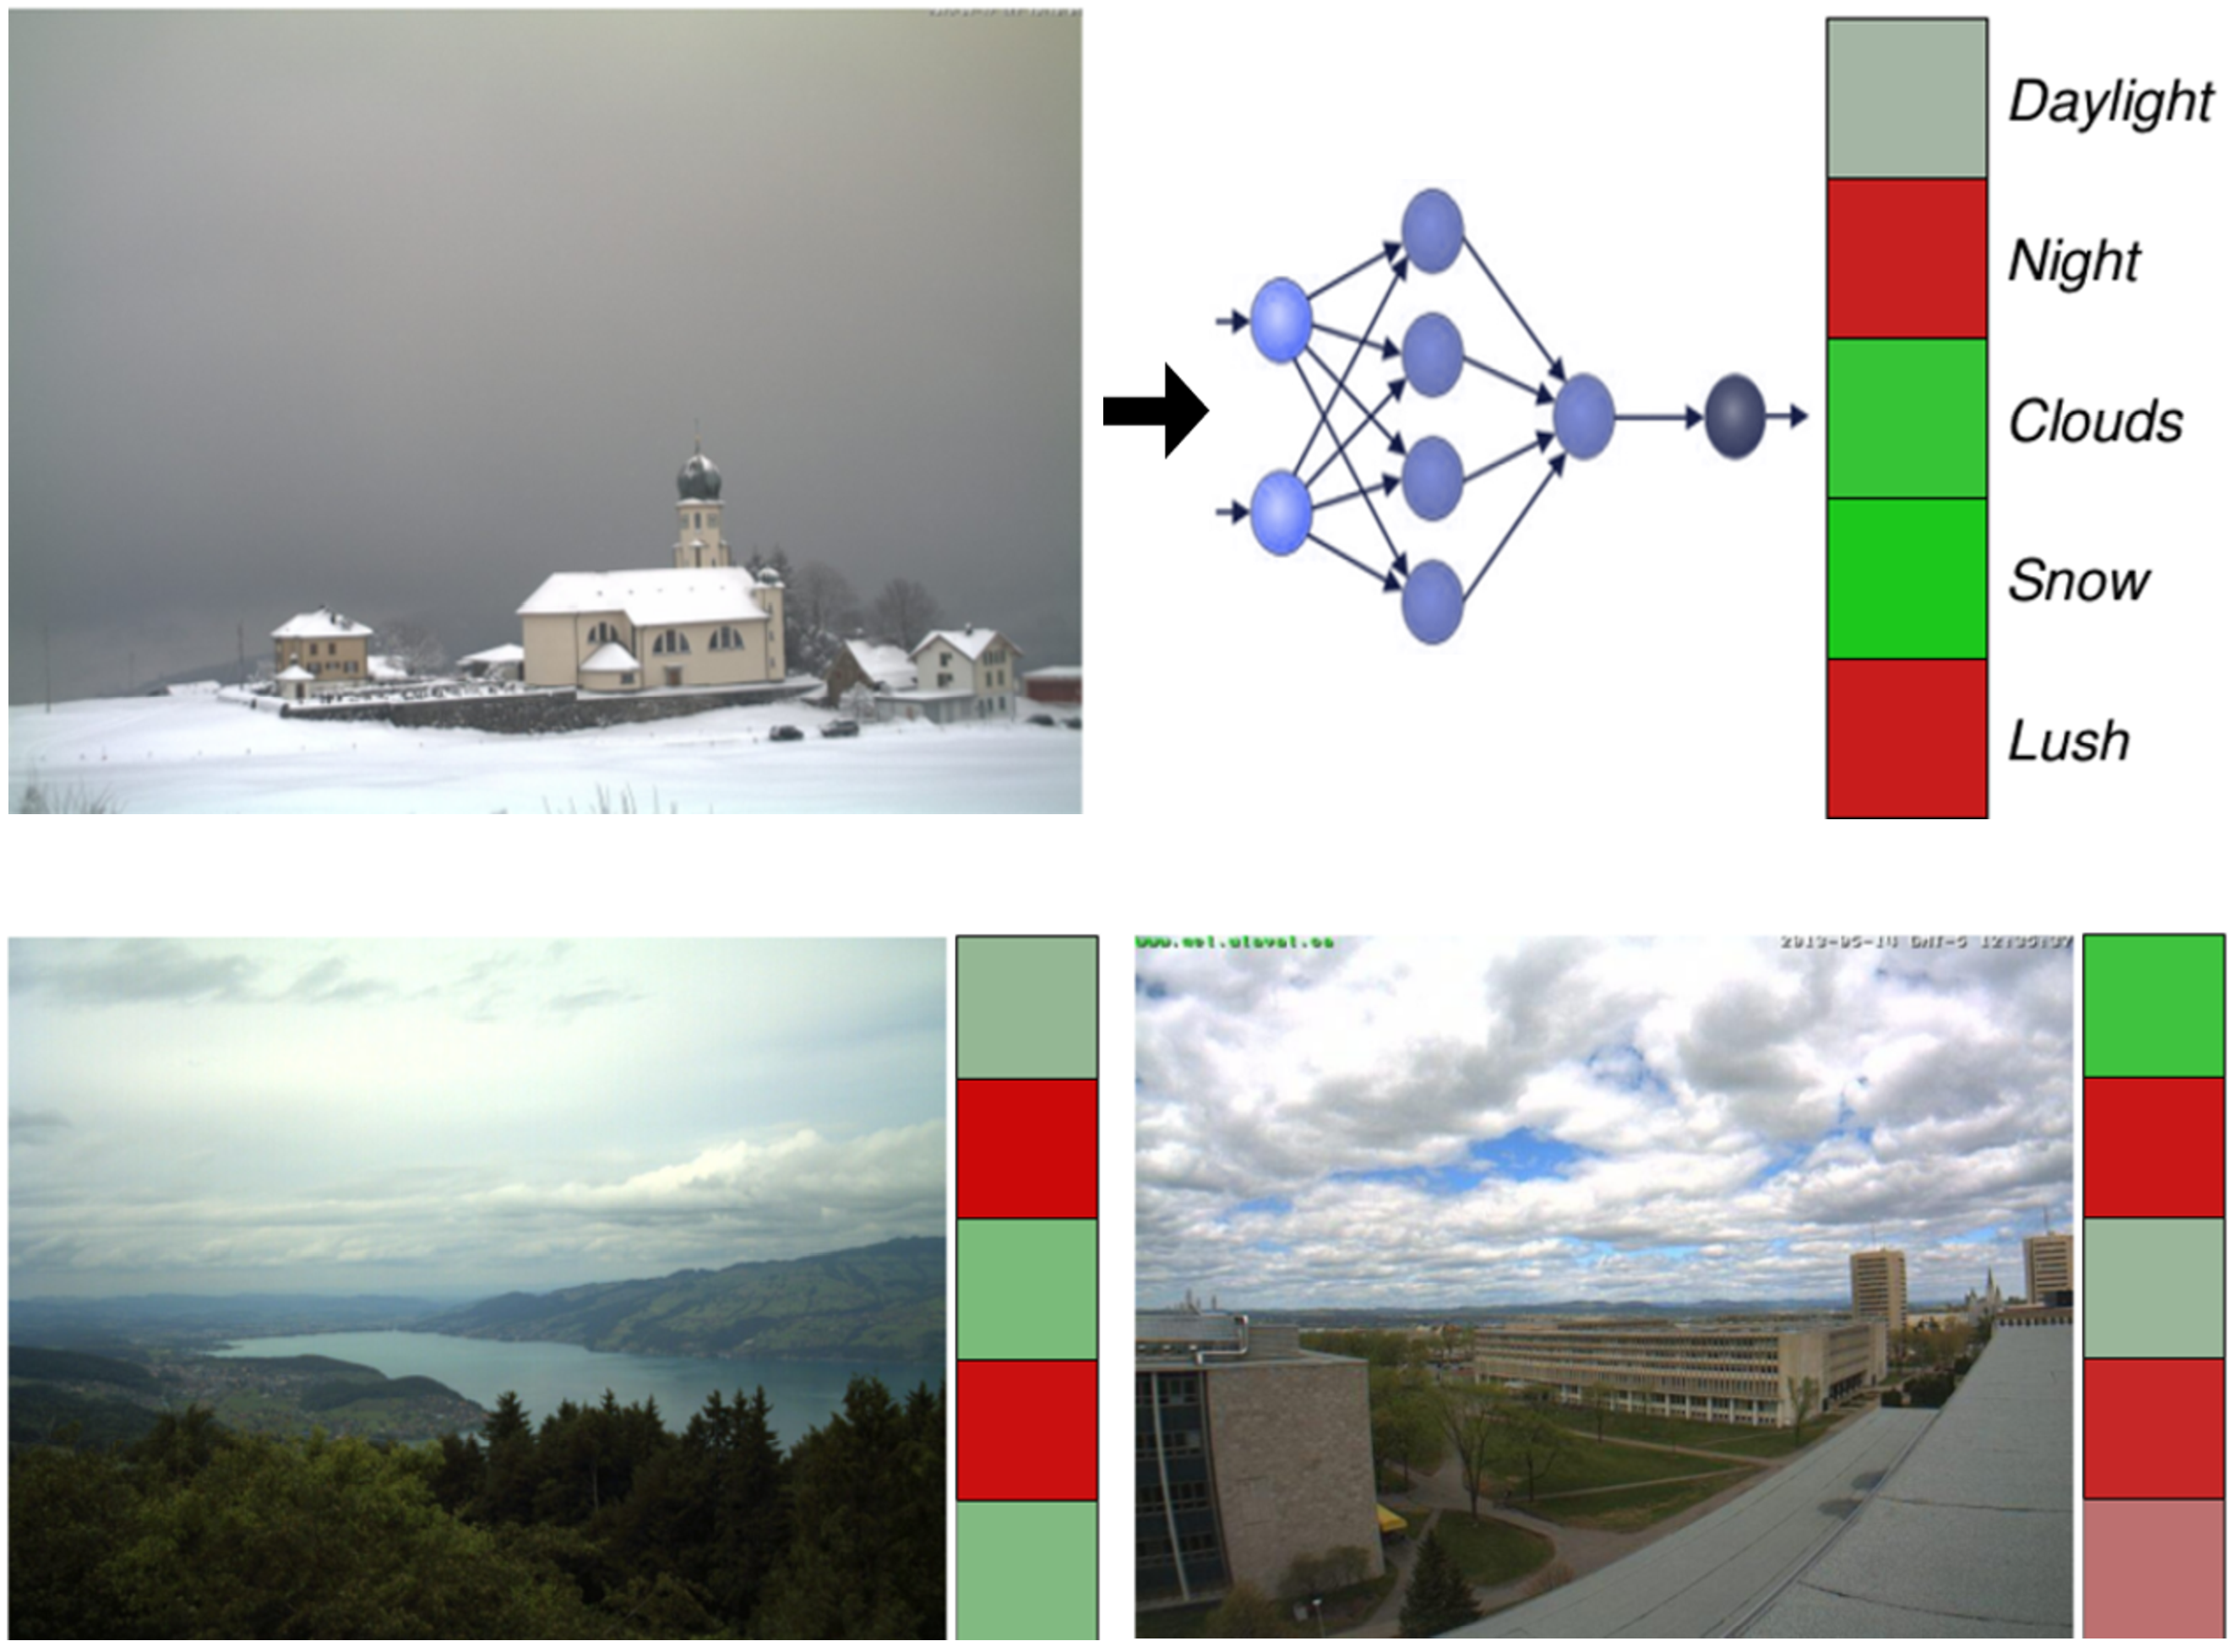
\includegraphics[width=0.5\textwidth, trim= 0mm 0mm 0mm 0mm]{figs/cartoon.pdf}
		\caption{This shows an overview of our proposed method and a subset of the
             output attributes.  In this case, red is a low attribute value and
             green is a high attribute value.}
		\label{fig:cartoon}
\end{figure}

%\begin{figure}
%	\centering
%		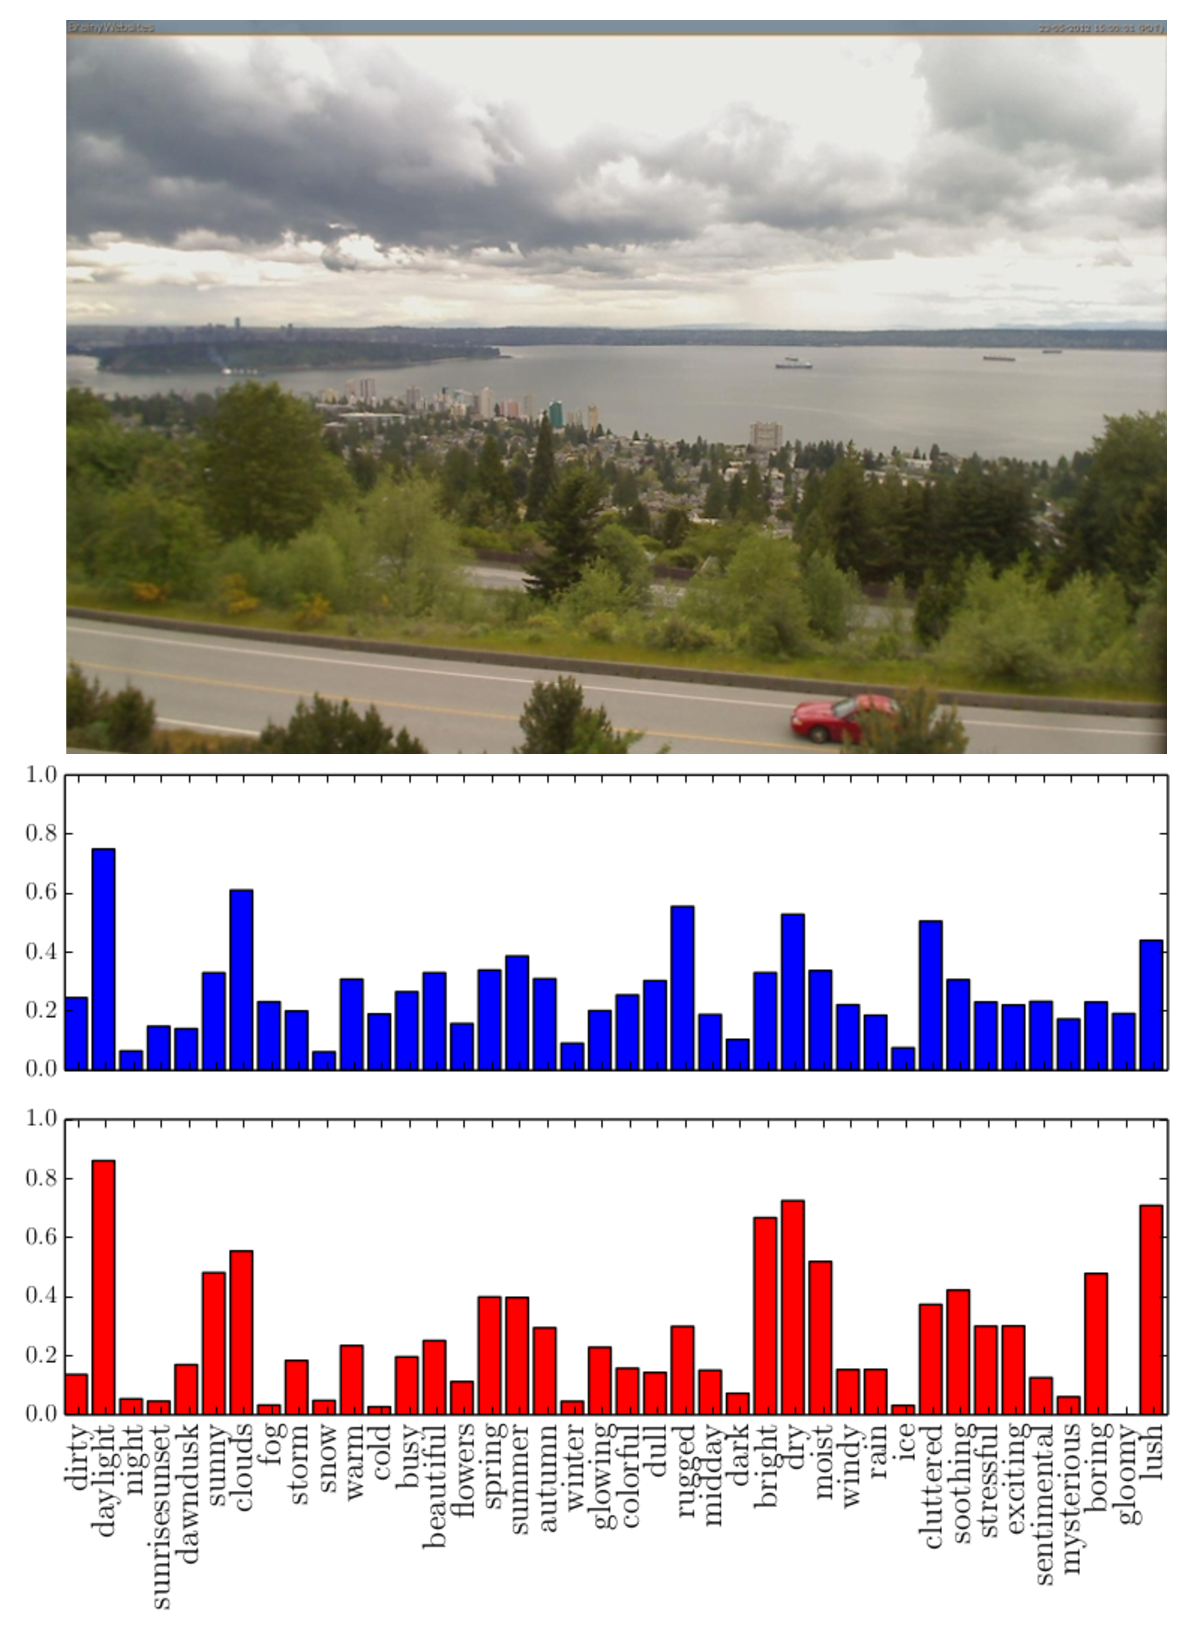
\includegraphics[width=0.5\textwidth]{figs/bars.pdf}
%		\caption{Example images from the Transient Attributes Dataset
%      with our network's confidence in each predicted label.
%      \todo{boring}}
%    \label{fig:results}
%\end{figure}

% what we can do now that we have this?

\todo{reword this}

The key contributions of this work are: 1) proposing several CNN network
training methods for predicting transient attributes, 2) a comprehensive
evaluation on two benchmark datasets~\cite{lutwoclass,Laffont14}, which shows
the speed and accuracy of the proposed networks, achieving state-of-the-art
performance, 3) releasing pre-trained networks for classifying transient scene
attributes in a popular deep learning framework~\cite{caffe14}, and 4)
demonstrating the real world utility of our methods for automatic webcam image
labeling. 

\subsection{Related Work}
Attributes are high-level descriptions of a visual property which offer some
additional semantic context for understanding an object, activity, or scene.
For example, a \emph{green} apple or a \emph{cloudy} day. Representations based
on such visual attributes have become increasingly popular in the vision
community as they offer the ability to to generalize across categories. The
first learning-based methods to take advantage of such high-level attributes
arose for the task of object
recognition~\cite{farhadi2009describing,lampert2009learning}, demonstrating the
power of learning by description. Many methods were quick to follow suit, with
applications ranging from content-based image
retrieval~\cite{siddiquie2011image} to characterizing facial
appearance~\cite{kumar2011describable}. Given their prowess, a significant
amount of research has focused on identifying useful
attributes~\cite{berg2010automatic} and crafting techniques to accurately
detect them in images~\cite{vedaldi2014understanding}. 

More recently, efforts have been made to adapt such attribute-based
representations for outdoor scene understanding, where the appearance of a
scene can change drastically over time.  Patterson and
Hays~\cite{patterson2012sun} constructed the SUN attribute dataset using
crowd-sourcing techniques to identify a taxonomy of 102 scene attributes from
human descriptions, designed to distinguish between scene categories. Lu et
al.~\cite{lutwoclass} use this dataset, along with two others, to classify
images as either sunny or cloudy.  Similarly, Laffont et al.~\cite{Laffont14}
introduced the Transient Attributes dataset, focused instead on perceived scene
properties and attributes that describe intra-scene variations. They defined 40
such attributes and presented methods for identifying the presence of those
attributes as well as applications in photo organization and high-level image
editing via attribute manipulation. 

To the best of our knowledge, we are the first to explore the application of
convolutional neural networks for learning transient scene attributes
using only raw image intensities as input.

\subsection{Background}

CNNs have been used extensively in recent
years to obtain state-of-the-art results on a wide variety of computer vision
problems.  In this work, we focus on a particular CNN architecture, often
called ``AlexNet'', introduced by Alex Krizhevsky et al.~\cite{caffenetnips12}
for single-image object classification. This network has eight layers with
trainable parameters: five convolutional layers (each connected, in a
feed-forward manner with pooling and dropout layers between each convolutional
layer) and three fully connected layers. Essentially, the convolutional layers
extract features from across the image and the fully connected layers combine
these features to obtain a score for each possible class. The final
classification decision is obtained by choosing the class with the highest
output score.

While this network architecture was originally developed for single-image
object classification, it has been shown to be adaptable to other problem
domains. If the new problem involves multi-class classification, all that is
needed is to modify the final fully connected layer to have the correct number
of output classes. Then, the network weights can be `fine-tuned' by running
iterations of stochastic gradient descent on the training data for the new
problem~\cite{yosinski2014transferable}.  The key is to start the optimization
with random weights for the new final layer and weights from an already trained
network for the other layers, for example using the weights from the original
AlexNet~\cite{caffenetnips12}, as an initial condition. If there is a large
amount of training data available for the new domain, it is also possible to
train the network from scratch by randomly initializing all
weights~\cite{zhou2014places}.  If the new problem domain is regression, not
classification, then the only change that is necessary is to change the network
loss function, perhaps replacing the SOFT-MAX loss with an $L_2$ loss.

\section{Estimating Transient Attributes with CNNs}
We propose the use of deep convolutional neural networks for estimating transient
scene attributes. We develop networks for two single-image problems: the
classification problem of estimating whether it is sunny or cloudy and a
collection of regression problems for representing the degree to which a large
number of transient attributes exist in the scene.  For each of these problems,
we use three different networks as starting conditions for optimization,
resulting in a total of six networks.  For both problems, we use the
``AlexNet'' CNN architecture, described in the previous section.  The remainder
of this section describes how we estimate network weights for each of these
networks.

% I don't know if we still need this plot.  It takes up 
% a lot of space and isn't terribly informative.  I think
% the space is better used by some of the other figures
\begin{figure*}[t!]
	\centering
		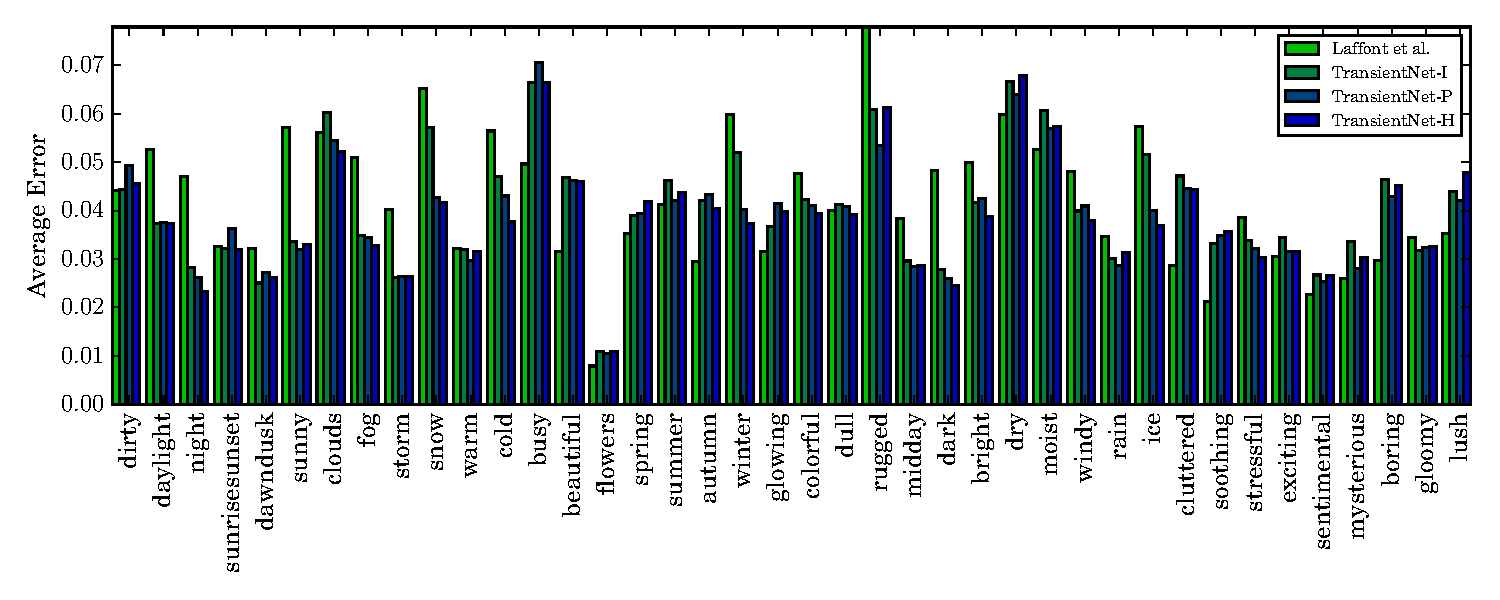
\includegraphics[width=1.0\textwidth, trim= 0 4mm 0 0]{figs/avg_err_compare.pdf}
		\caption{This shows the average errors for each attribute from the method proposed
						 by Laffont et al., and our three networks: TransientNet-I, TransientNet-P,
             and TransientNet-H.  TransientNet-H has the lowest average error for a 
             majority of the attributes.}
		\label{fig:compare}
\end{figure*}

\textbf{CloudyNet:} For the problem of classifying whether an image is sunny or
cloudy, we use the data provided by Lu et al.~\cite{lutwoclass} to train our
network, which we call CloudyNet.  We follow their protocol for
generating a train/test split: we randomly shuffle sunny/cloudy images
and then select 80\% of each class for training and 20\% for testing.
This process is repeated five times resulting in five random 80/20
splits of the data. During evaluation we report the mean and variance
of normalized accuracy using five fold cross validation. The only
modification to the network architecture that was required was
dropping unnecessary output nodes from the final fully connected layer
(in the end we have two output nodes).

\textbf{TransientNet:} For the more challenging problem of estimating
the presence of a broad range of attributes in an image, we take
advantage of the attributes and associated dataset introduced by Laffont
et al.~\cite{Laffont14}. The authors define a set of 40 transient attributes
(see \figref{compare} for the full list of attributes), each of which is
assigned a value between zero and one, representing the confidence
of that attribute appearing in an image. We use the same holdout
train/test split in which images from 81 static outdoor webcams are
used for training and images from a distinct set of 20 other webcams are
used for testing.  In this scenario, we modify the network architecture
by changing the final fully connected layer to have 40 output nodes, one for
each transient attribute, and updating the loss function to an $L_2$
loss. 

For each network, we train starting from three different initial conditions,
resulting in six distinct sets of network weights. The first set of initial
conditions are taken from a network that was was trained for object
classification on 1.2 million images from the ImageNet ILSVRC-2012
challenge~\cite{ILSVRCarxiv14}.  We call the networks that result from this
fine-tuning process CloudyNet-I and TransientNet-I.  The second set of initial
conditions were taken from a network~\cite{zhou2014places} that was trained for
scene classification on 2.5 million images with labels in 205 categories from
the Places Database~\cite{zhou2014places}. We call the resulting networks
CloudyNet-P and TransientNet-P.  The final set of initial conditions were taken
from a network~\cite{zhou2014places} that was trained for both object and scene
classification.  This hybrid network was trained on a combination of the Places
Database~\cite{zhou2014places} and images from the training data of ILSVRC-2012
challenge~\cite{ILSVRCarxiv14}.  The full training set contained 205 scene
categories from the Places Database and 978 object categories from ILSVRC-2012
totaling about 3.6 million images.  We call the resulting networks CloudyNet-H
and TransientNet-H.

%\textbf{Expanded Dataset:} We expand the Transient Attributes dataset from
%Laffont et al.~\cite{Laffont14} using AMOS~\cite{jacobs07amos} webcams.  We
%first find the geolocation of the AMOS webcams within the transient attributes
%dataset.  Images from cameras with locations near these webcams are downloaded.
%Images from nearby webcams with corresponding timestamps to images in the
%Transient Attributes Dataset are assigned the ground truth labels from the
%dataset.  This is based on the idea that nearby webcams should have similar
%transient attributes at any given time. 
%\todo{get more specifics from Ted} 
%
%\textbf{Partial Siamese TransientNet:}

\textbf{Implementation Details:} Our networks are trained using the
Caffe~\cite{caffe14} deep learning framework, the CaffeNet reference network
architecture (a variant of AlexNet), and pre-trained networks
from the Caffe Model
Zoo\footnote{\url{http://caffe.berkeleyvision.org/model_zoo.html}}.
All of our networks were trained on NVIDIA M2075 GPU Cards for 24
hours each, and evaluated using Caffe in CPU mode on Dell C6220
Servers equipped with Dual Intel E5-2670 8 Core (Sandy Bridge)
processors at 2.6 GHz.  The full network optimization definition, the
final network weights, and the output from our methods will be made
available online for all six networks \emph{pending publication}.

\section{Evaluation}
%\todo{there isn't enough emphasis on how much faster this method is
%than the others... make explicit comparisons (maybe a table)}
We evaluate the six networks defined in the previous section on two large-scale
benchmark datasets. The results show that these deep networks obtain
state-of-the-the-art results. 


\subsection{Two-Class Weather Classification}
\todo{the following intros are weird because you have already said which
datasets you used for training}
In our first experiment, we use the dataset created by Lu et
al.~\cite{lutwoclass} to train our networks for two class weather
classification.  The dataset contains images collected from the SUN
Database~\cite{xiaoSUN}, the LabelMe Database~\cite{russell2008labelme}, and
Flickr. The dataset contains 5000 sunny and 5000 cloudy images. Flickr images
were collected manually by ``helpers'' unaware of the purpose or methods of Lu
et al. The dataset was then pruned for images with similar histograms, and
finally pruned by another round of helpers to narrow the dataset to 10,000
images.  \tblref{twoclass} shows the normalized accuracies of our networks
compared to the method proposed by Lu et al~\cite{lutwoclass}.  The normalized
accuracy was calculated by $ \max\{((a - 0.5) / 0.5), 0\} $, where $a$ is the
traditionally obtained accuracy. All three of the networks outperform the state
of the art for two class weather classification with CloudyNet-H predicting the
most accurately.  CloudyNet-H averages 0.0672s per image for prediction. 

\subsection{Transient Attributes}
We used the dataset created by Laffont et al.~\cite{Laffont14} to train our
networks for transient attribute prediction. The dataset contains images from
outdoor webcams in the Archive of Many Outdoor Scenes~\cite{jacobs07amos} and
the Webcam Clip Art Dataset~\cite{lalondesig09}.  The webcams span a wide range
of outdoor scenes, from urban regions to wooded, mountainous regions. Each
webcam has 60--120 representative images that feature variations in weather,
lighting conditions, etc.  The images are high resolution and are aligned to a
reference frame through a homography warp with manually specified
correspondences.  The final dataset consists of 8571 images from 101 webcams.

\figref{compare} shows the average errors from TransientNet-I, TransientNet-P,
TransientNet-H and Laffont et al. for each attribute in the dataset.
TransientNet-H performs best on more than half of the attributes and is the
best performing CNN that we trained.  TransientNet-H has the lowest overall
average error as shown in \tblref{transient}.  TransientNet-P and
TransientNet-H have similar performance, mostly due to them being pretrained on
similar sets of data.

\tblref{timing} compares the average prediction speed for the method provided
by Laffont et al.~\cite{Laffont14} and our best performing network,
TransientNet-H.  Laffont et al.'s method takes an average of 3.486 seconds to
label a single image.  Our network takes an average of 0.192 seconds to label a
single image.  Labeling a million images using Laffont et al.'s method on a
single machine would take upwards of 40 days, whereas our network on a single
machine would take approximately 2.2 days. This number is easily reduced
through simple distributed processing, though.  This 18x speed up allows for
large scale, real world applications of the transient attributes.


%\todo{edit this text to not talk about rel err plot}
%
%\figref{relerr} shows the relative error between our method using
%TransientNet-H and the method presented by Laffont et al.~\cite{Laffont14}  The
%average relative error for each attribute using the method by Laffont et al.\
%was subtracted from the average relative error using TransientNet-H.  A
%negative value means TransientNet-H had a smaller error and a positive value
%means Laffont et al. had a smaller error.  For example, the difference between
%the two methods on the attribute \emph{night} was around 2.5 percentage points,
%with TransientNet-H having the smaller error.  TransientNet-H averages 0.0699s
%per image for prediction. 

\begin{table}[t]
	\centering
	\caption{Two class weather classification accuracy}
	\begin{tabular}{ | l | c | }
		\hline
			Method & Normalized Accuracy \\ \hline \hline
			Lu et al.~\cite{lutwoclass}& $ 53.1 \pm 2.2 $ \\ \hline
			CloudyNet-I & $ 85.72 \pm 0.527 $ \\ \hline
			CloudyNet-P & $ 86.18 \pm 0.572 $ \\ \hline
			CloudyNet-H & $ \textbf{87.14} \pm 0.263 $ \\ 
		\hline
	\end{tabular}
	\label{tbl:twoclass}
\end{table}

\begin{table}[t]
	\centering
	\caption{Transient attribute prediction errors}
	\begin{tabular}{ | l | c | }
		\hline
			Method & Average Error \\ \hline \hline
			Laffont et al.~\cite{Laffont14}& 4.2\% \\ \hline
			TransientNet-I & 4.05\% \\ \hline
			TransientNet-P & 3.87\% \\ \hline
			TransientNet-H & \textbf{3.83\%} \\ 
		\hline
	\end{tabular}
	\label{tbl:transient}
\end{table}

\begin{table}[t]
	\centering
	\caption{Transient attribute prediction speed}
	\begin{tabular}{ | l | c | }
		\hline
			Method & Average Prediction Speed \\ \hline \hline
			Laffont et al.~\cite{Laffont14}& $ 3.486 s $ \\ \hline
			TransientNet-H & $ \textbf{0.192 s} $ \\ 
		\hline
	\end{tabular}
	\label{tbl:timing}
\end{table}

%\begin{figure}[t!]
%  \renewcommand{\arraystretch}{1.6}
%  \centering
%  \begin{tabular}[b]{| c | c |}
%    \hline
%    Image & Labels \\
%    \hline \hline
%    \multirow{3}[3]{*}[-2mm]{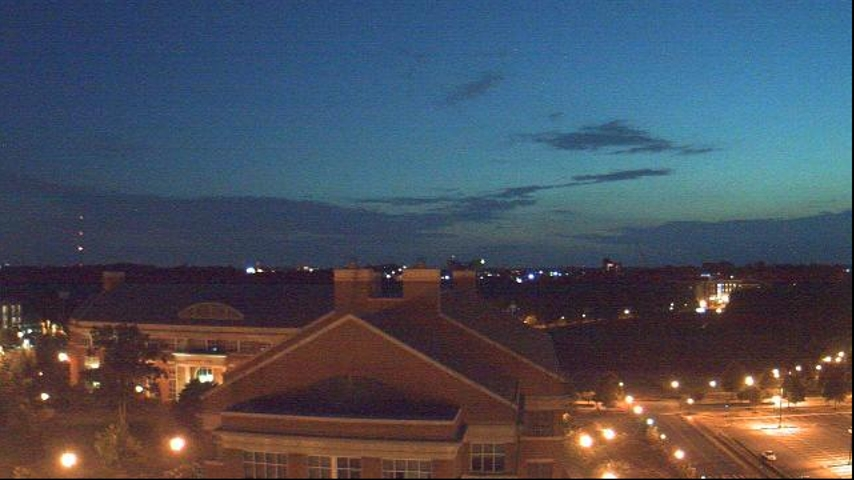
\includegraphics[width=0.19\textwidth]{figs/labels_1.jpg}}
%      & night, not sunny \bigstrut \\
%      & dark, not snow \bigstrut  \\
%      & glowing, not midday \bigstrut  \\
%    \hline
%    \multirow{3}[3]{*}[-1mm]{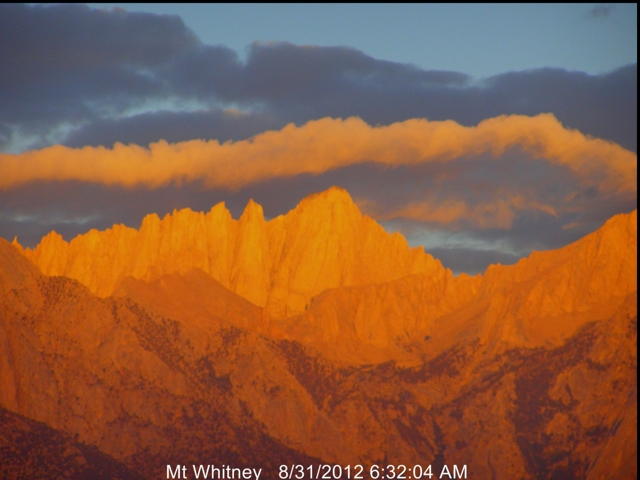
\includegraphics[width=0.17\textwidth]{figs/labels_2.jpg}}
%      & rugged, not flowers \bigstrut  \\
%      & dawndusk, not rain \bigstrut  \\
%      & sunrisesunset, not storm  \bigstrut \\
%    \hline
%  \end{tabular}
%  \caption{Example labels for images using TransientNet-H}
%  \label{fig:labels}
%\end{figure}

% I think we could do without this plot as well.  At the very least
% we should get rid of this plot or the bigger bar chart
%\begin{figure}[t!]
%	\centering
%		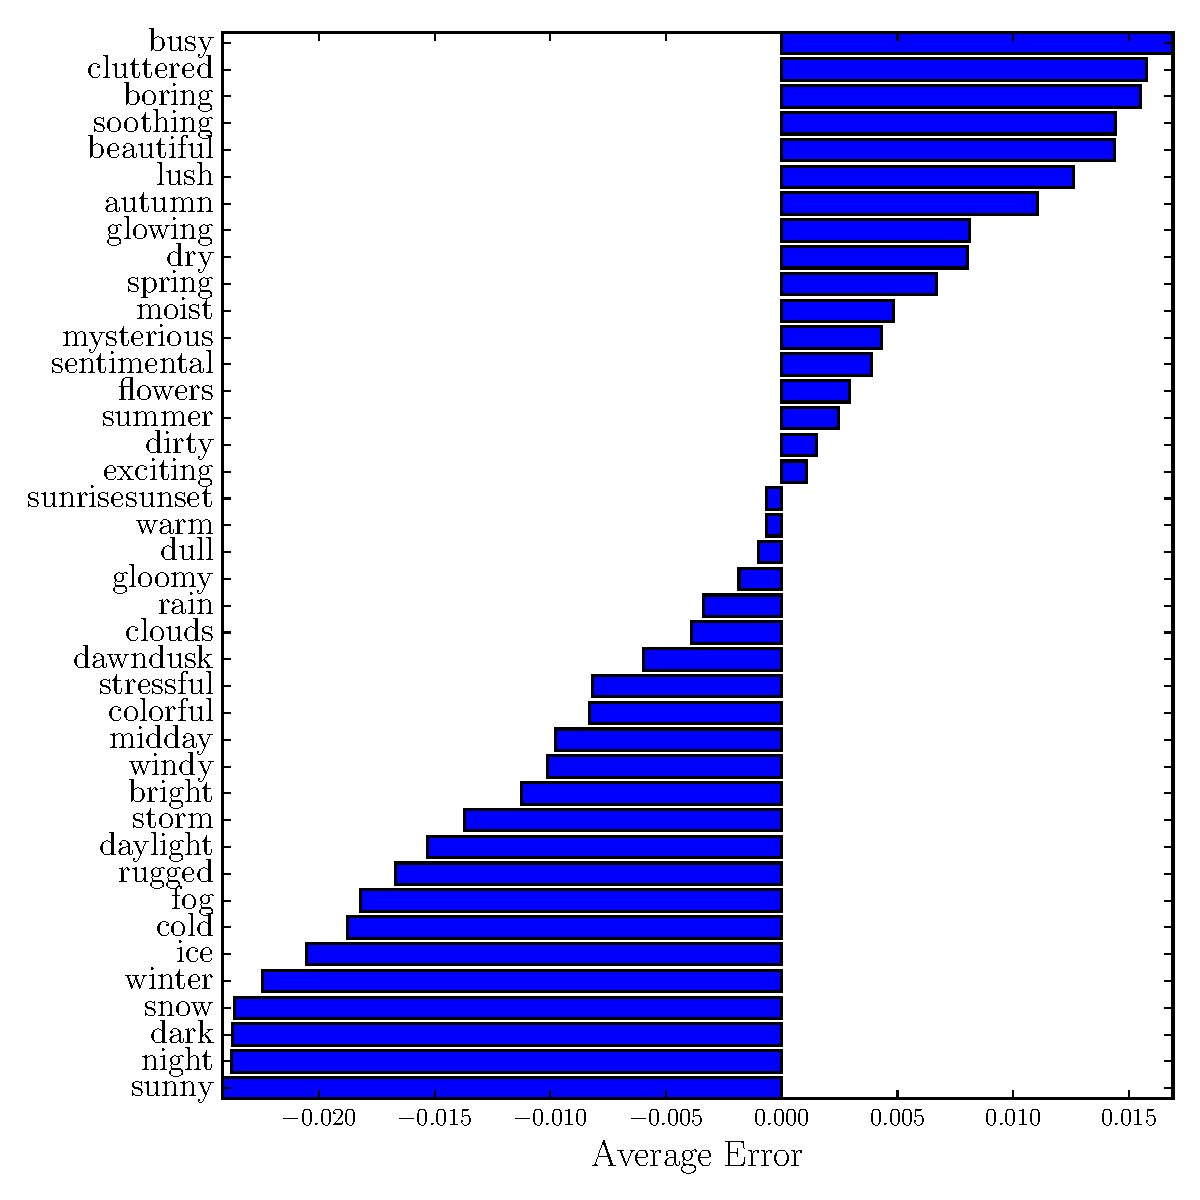
\includegraphics[width=0.5\textwidth]{figs/rel_err_cmr.pdf}
%		\caption{This shows the relative errors of TransientNet-H against the method 
%						 proposed by Laffont et al. for each attribute.  Attributes with a 
%						 negative average error are attributes that are predicted more 
%						 accurately by our method.}
%		\label{fig:relerr}
%\end{figure}

\begin{figure}[t]
	\centering
		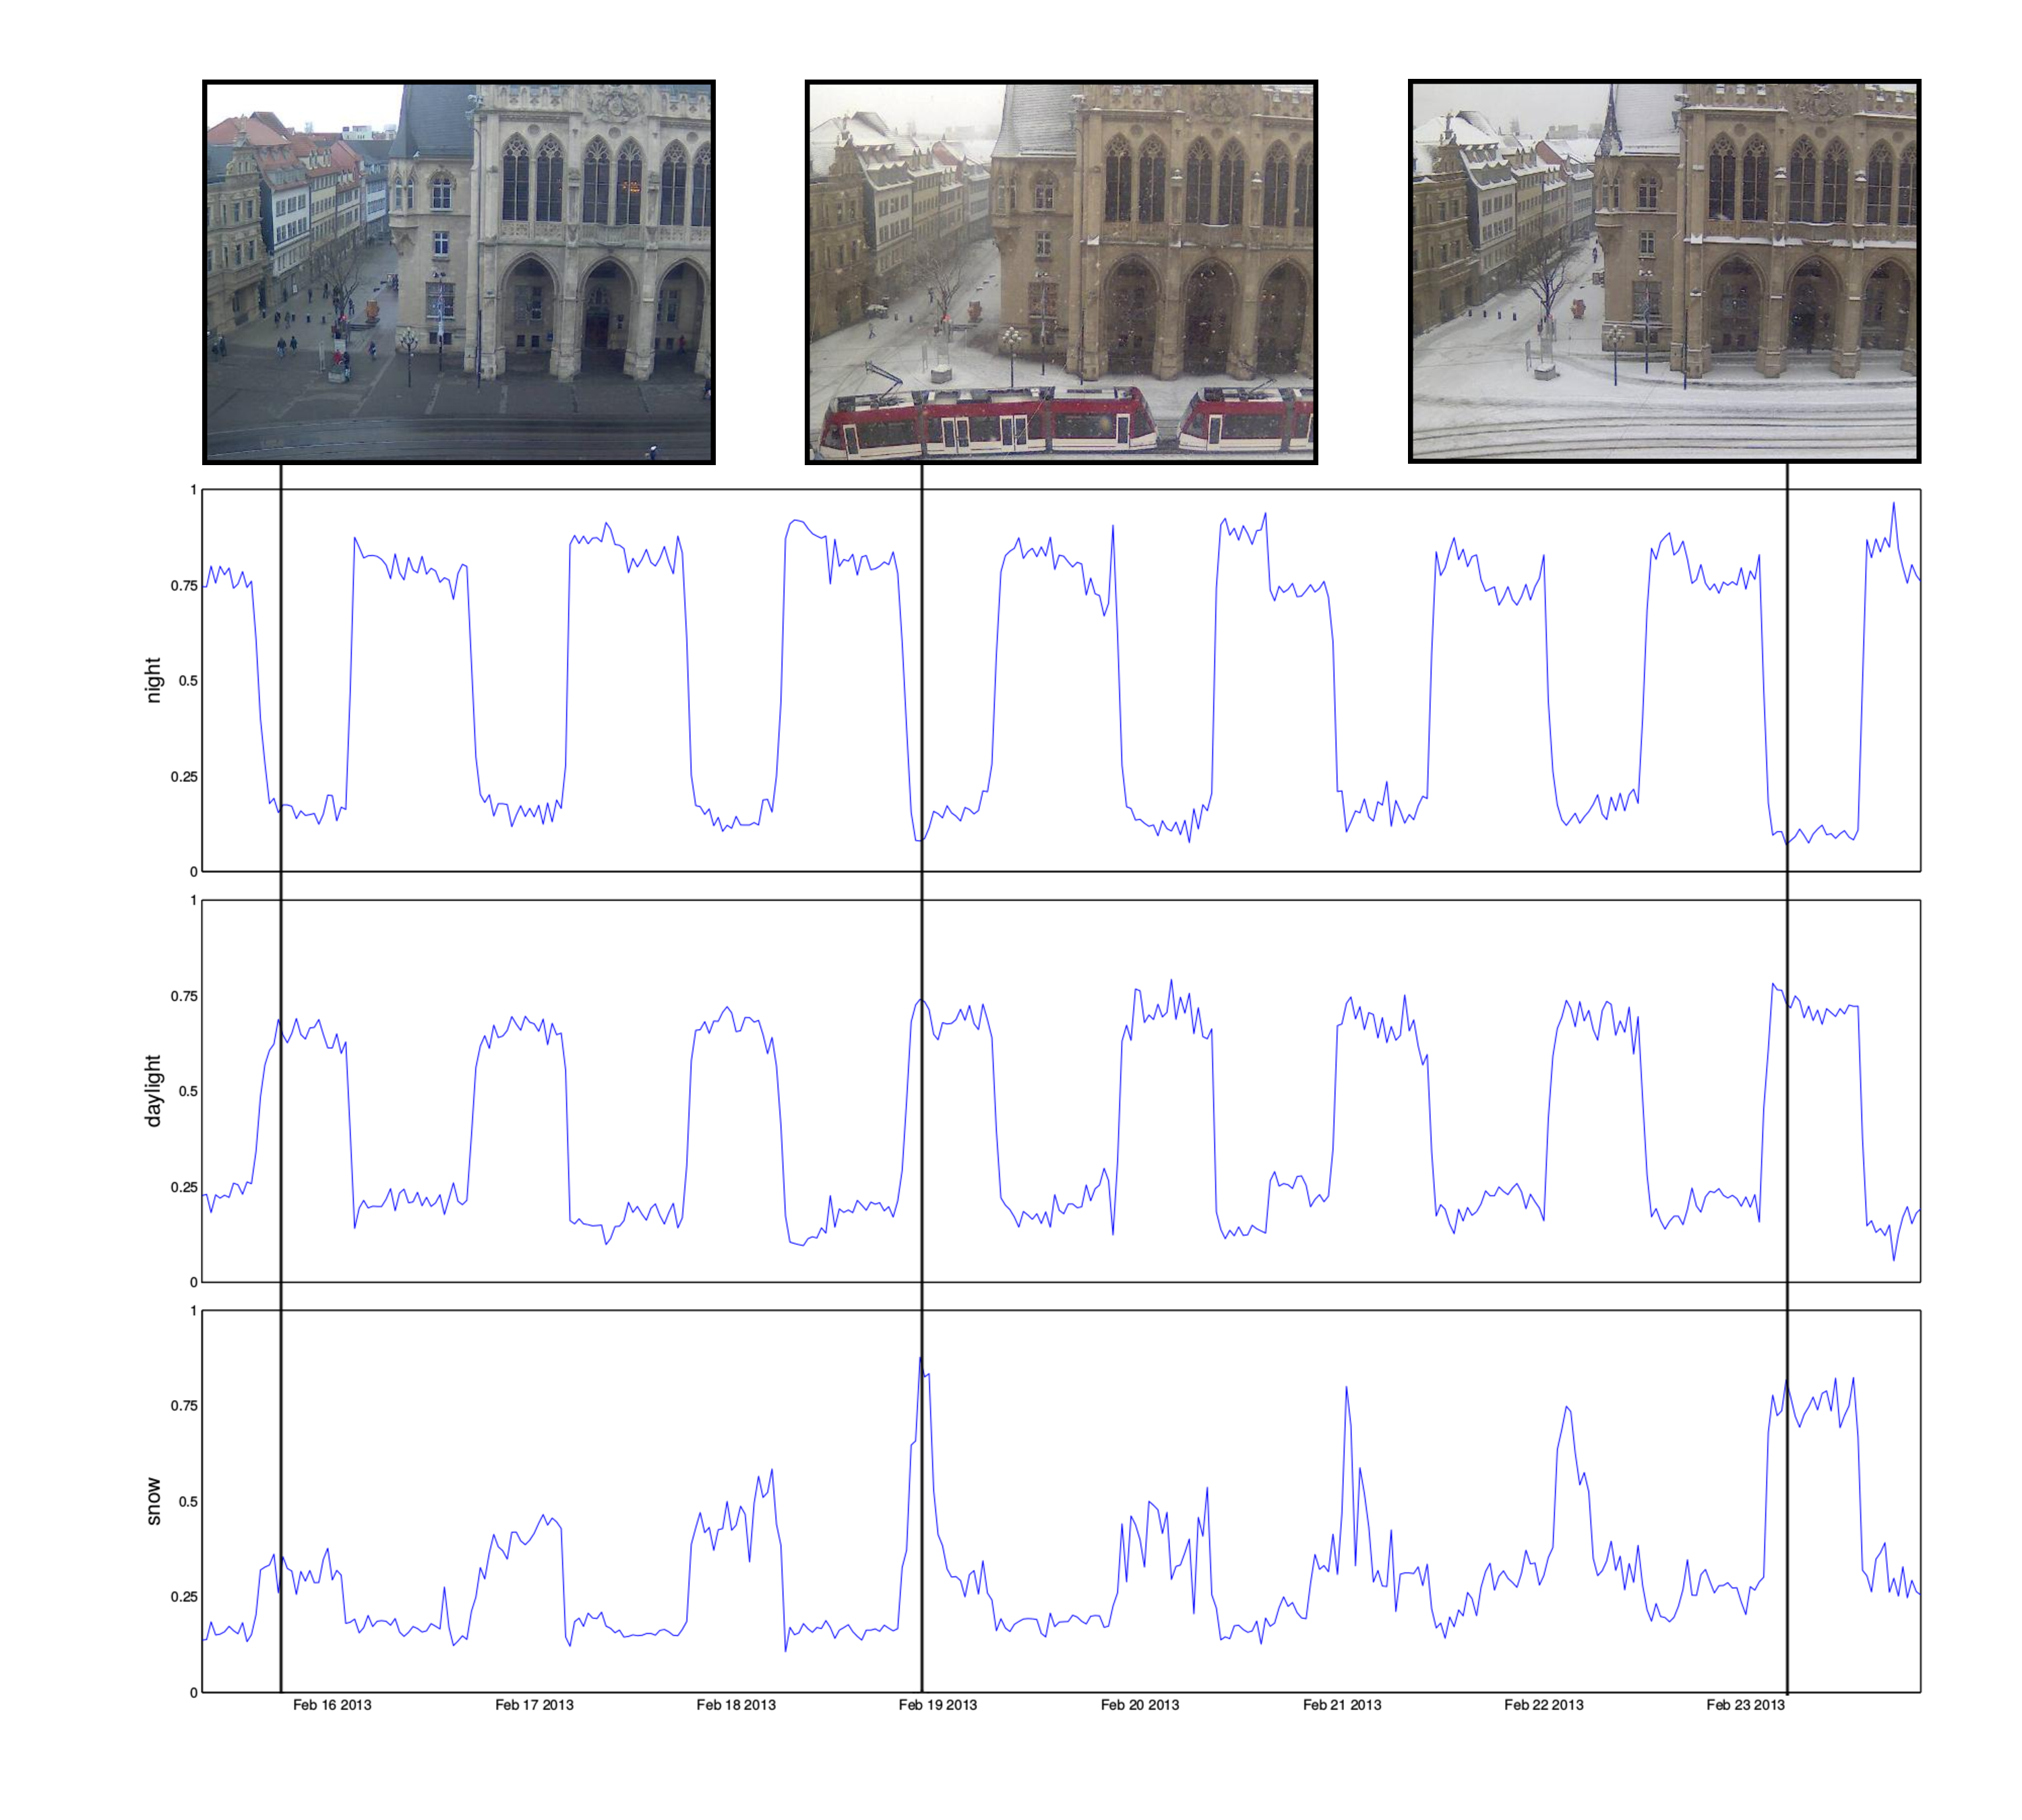
\includegraphics[width=0.5\textwidth, trim= 5mm 15mm 0mm 10mm]{figs/attr_compare.pdf}
		\caption{This shows a snapshot of three attributes over a week of data for
             an AMOS webcam.  The example images show that our network 
             correctly labels snowy scenes.}
		\label{fig:attrcmp}
\end{figure}

\begin{figure}[t]
	\centering
		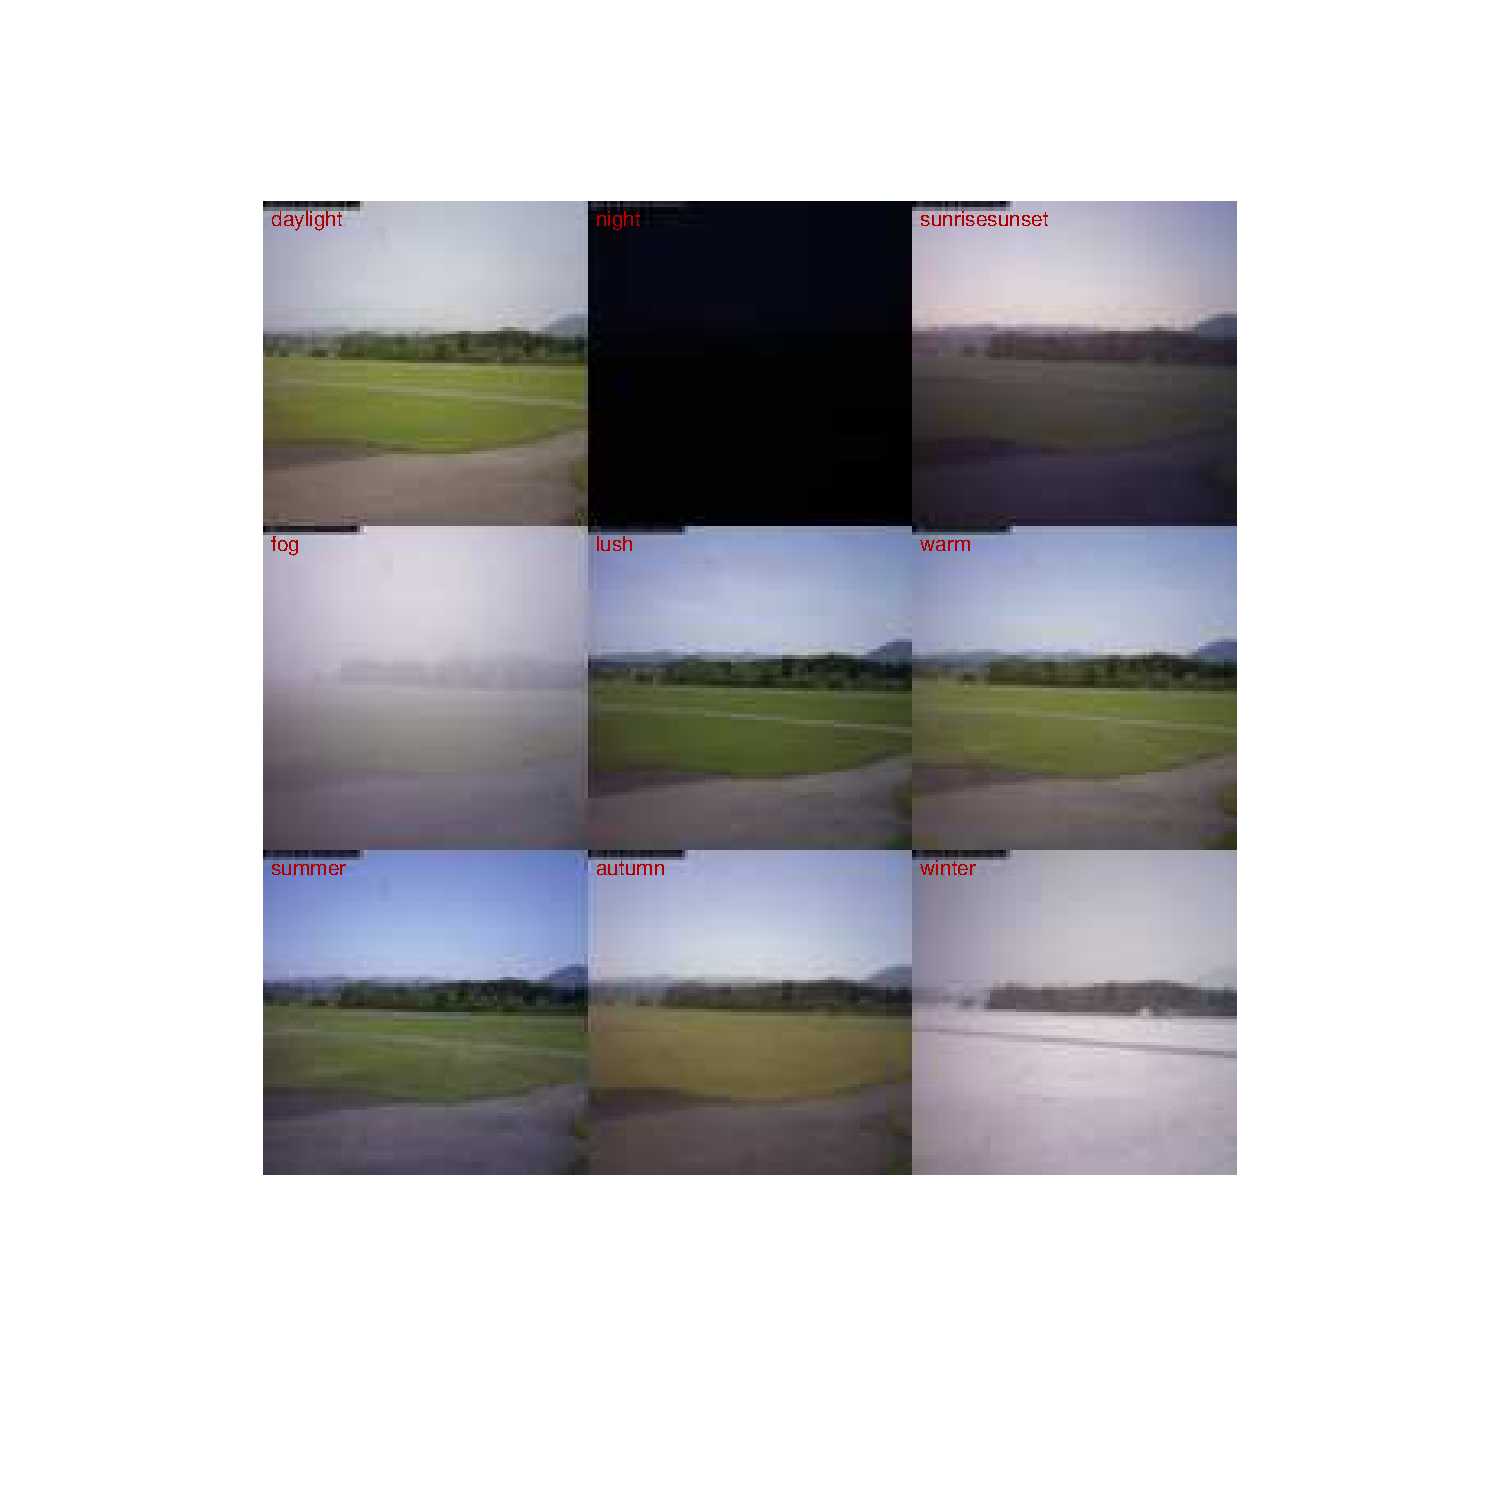
\includegraphics[width=0.5\textwidth, trim= 35mm 50mm 30mm 31mm]{figs/montage_pruned_cam_7211.pdf}
		\caption{This shows the average of the 100 most confident images for
             a subset of transient attributes from a given webcam.} 
		\label{fig:netvis}
\end{figure}

\begin{figure*}
  \centering
  \begin{subfigure}[b]{0.49\textwidth}
    \centering
		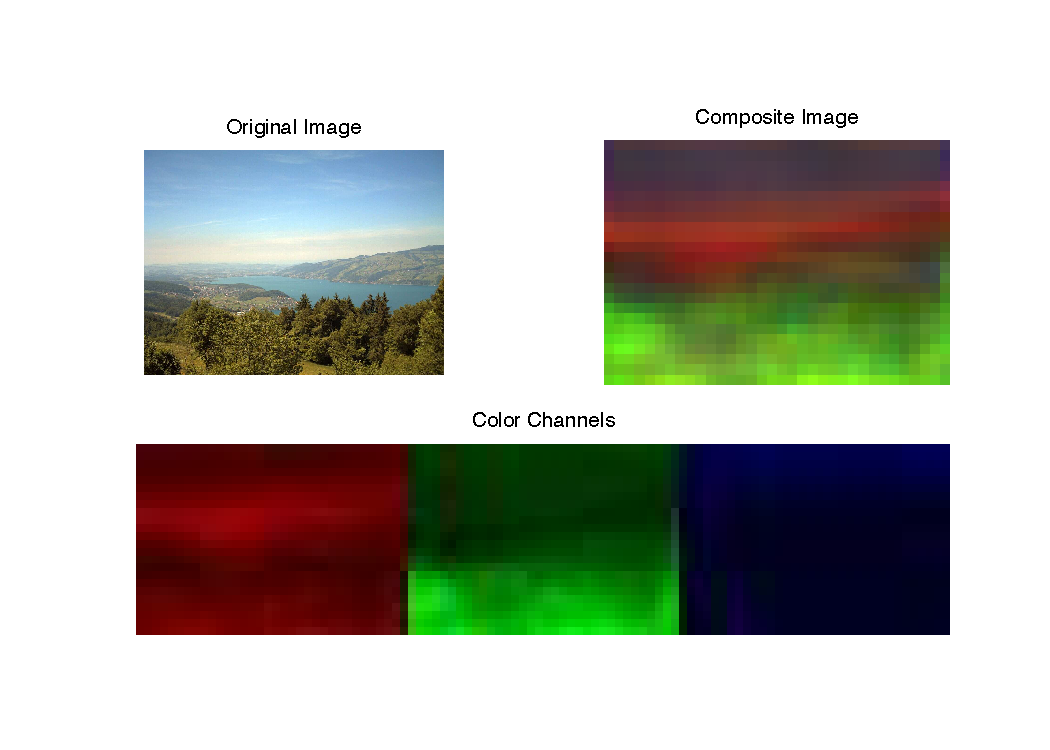
\includegraphics[width=\textwidth, trim= 15mm 17mm 10mm 10mm]{figs/false_color_7371.pdf}
    \caption{RGB = [\textit{sunny, lush, snow}]}
    \label{fig:false_color_1}
  \end{subfigure}
  \begin{subfigure}[b]{0.49\textwidth}
    \centering
		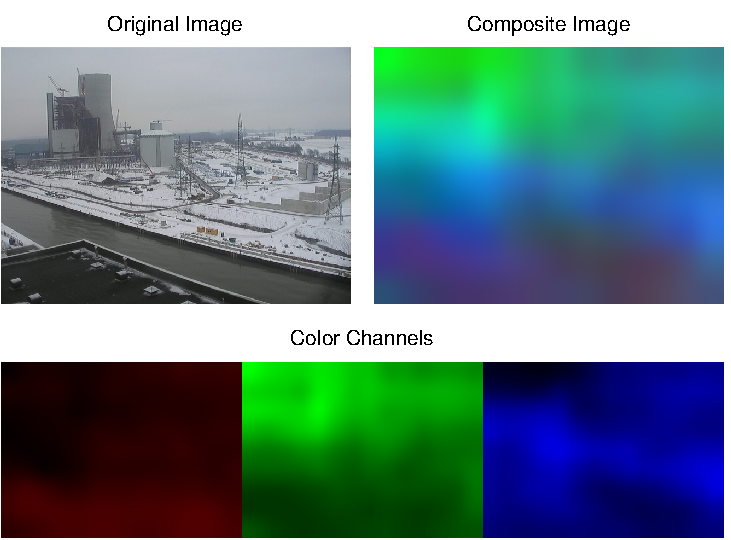
\includegraphics[width=\textwidth, trim= 15mm 17mm 10mm 10mm]{figs/false_color_82.pdf}
    \caption{RGB = [\textit{sunny, storm, snow}]}
    \label{fig:false_color_2}
  \end{subfigure}
  \caption{This shows example images run through the fully convolutional
           TransientNet-H with different attributes as the color channels for
           the composite image.}
  \label{fig:false_color_ims}
\end{figure*}


\section{Application to Automatic Webcam Image Labeling}

The speed gained using our network allows us to apply transient attributes to
real world data.  We discuss how the attributes change over time and look at
the most confident images per attribute for webcam data.  We then propose a
method for automatically labeling images from outdoor webcams, allowing for
advanced searching of webcam collections, such as AMOS~\cite{jacobs07amos}. We
also use labeled webcam images to create year-long summaries of transient
attributes for a webcam.

\subsection{Time Series and Scene Analysis}

We look at the values for selected attributes over a given span of time and
their corresponding webcam images.  We qualitatively confirm the predicted
attribute values and visualize the scene which maximizes each attribute.
\figref{attrcmp} shows the time series for three selected attributes
(\textit{night, daylight, and snow}) from an AMOS~\cite{jacobs07amos} webcam
over the period February 16th, 2013 to February 23rd, 2013.  The correspondence
between the \textit{daylight} and \textit{night} time series can be clearly
seen in this Figure.  The peaks in one correspond to the valleys in the other
and vice versa.  \figref{attrcmp} also shows snapshots of the scene from points
along the time series.  The snapshots show correctly labeled snowy periods in
the scene as well non-snowy periods.

\figref{netvis} visualizes the top scoring images from a single
AMOS webcam across a subset of the transient attributes.
100 images with the highest score for each attribute (per the \textit{fc8}
output layer) were averaged to create the images in \figref{netvis}.  The
subset of attributes shown in \figref{netvis} represent a wide variety of
conditions of the scene.  The seasonal attributes (\textit{autumn, summer,
winter}) show how the scene changes throughout the year and lighting attributes
(\textit{sunrise/sunset, daylight, night}) shows the scene in various lighting
conditions.  Other attributes not shown in this montage have similar average
images to the ones shown, (\textit{e.g., glowing and colorful similar to
sunrise/sunset, windy and rain similar to fog}).  This suggests that the
network may not distinguish between these attributes well or that these
attributes have some correlation with each other.

\begin{figure}[t]
	\centering
		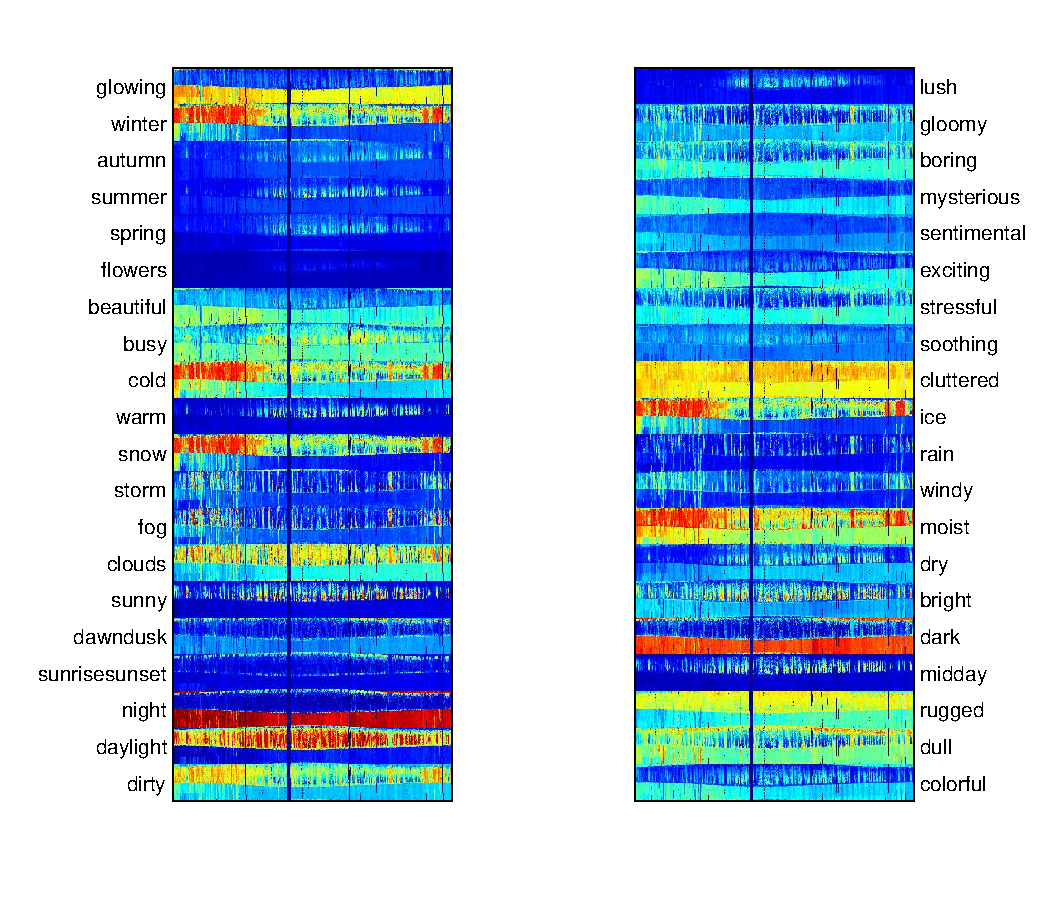
\includegraphics[width=0.5\textwidth, trim= 5mm 15mm 0mm 10mm]{figs/summary_260.pdf}
		\caption{This shows the transient attribute values for a year of webcam 
             data.  Each column corresponds to a day of the year and each row
             corresponds to a time of day.}
		\label{fig:webcam_summary}
\end{figure}

\subsection{Labeling and Summarizing a Webcam}

Webcam collections such as AMOS~\cite{jacobs07amos} contain thousands of
geolocated webcams with years of archived data.  Searching for scenes with a
set of desired attributes is usually done by manually looking through lists of
webcams and images.  TransientNet simplifies this process by using output
scores to tag images and webcams with certain attributes.  If an attribute is
above a defined threshold, the image is labeled with that attribute.  The
opposite is true as well.  If an attribute is below a defined threshold, the
attribute is added to a list of attributes the image does not have.  This
enables users to use queries such as ``sunny'' or ``not winter''.  Labeling is
done on the image level as well as the webcam level.  Attributes that
frequently have high values in a webcam (aside from daylight, night, etc) are
used to tag the webcam.  A labeling scheme like this one allows a user to
search for the snowy images from a \textit{mysterious} webcam. This allows for
easier searching of large collections of webcams.

We create summaries of the transient attributes for webcams using images pushed
through TransientNet.  Each column in the summary is a single day and each row
a different time of the day (in 30 minute intervals).  Each pixel is colored
based on the attribute value for the corresponding webcam image.
\figref{webcam_summary} shows all 40 attribute summaries for an AMOS webcam.
Attributes such as \textit{snow}, \textit{cold}, \textit{winter}, etc. have
higher values in the winter months and lower values during the summer months.
The \textit{night} and \textit{daylight} attributes clearly show the day/night
cycle for the location of the image.  Properties about the scene can be
inferred from these summaries.  Consistently high values for the
\textit{glowing} attribute at night indicate the presence of streetlights
and/or other man made light sources in the scene.

\subsection{Visualizing Attributes}
\todo{better title for this subsection}

We convert the the final, fully connected layers of TransientNet to be
convolutional with the same number of outputs.  The output from this new,
''fully convolutional'' network allows us to create images showing an
attribute's value across an input image.  \figref{false_color_ims} shows two
examples of this.  The values for each attribute can be visualized in a single
channel image.  Combining three of these images results in the composite
images.  \figref{false_color_1} shows a composite image using the
\textit{sunny}, \textit{lush}, and \textit{snow} attributes as the color
channels.  As expected, there are no snowy areas in the input image, shown
in the blue channel, and the bottom of the image contains high values for the
lush attribute, shown in the green channel.  The sunny attribute is higher 
towards the horizon and middle of the sky, show in the red channel, possibly 
due to the sky being brighter in these regions.  \figref{false_color_2} shows
a composite image using the \textit{sunny}, \textit{storm}, and \textit{snow}
attributes as the color channels.  The image has low values for the sunny
attribute, shown in the red channel, and high values for the storm attribute,
show in the green channel.  The storm attribute is higher towards the top
of the image in the overcast sky.  The snow covered ground from the 
snow-storm appears in blue channel with high values for the snow attribute in
the middle of the image.

\begin{figure*}
  \centering
  \begin{subfigure}[b]{0.33\textwidth}
    \centering
		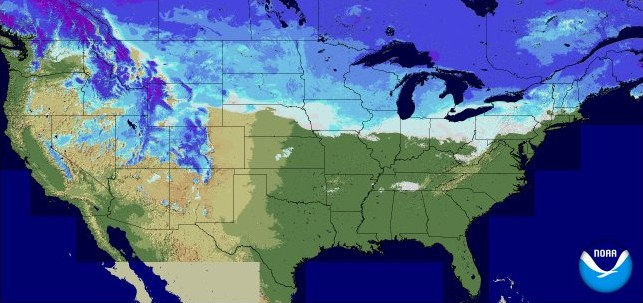
\includegraphics[width=\textwidth, trim= 0mm 0mm 0mm 0mm]{figs/snow_gt_1.jpg}
    \caption{January 1st, 2014}
    \label{fig:snow_map_1}
  \end{subfigure}
  \begin{subfigure}[b]{0.33\textwidth}
    \centering
		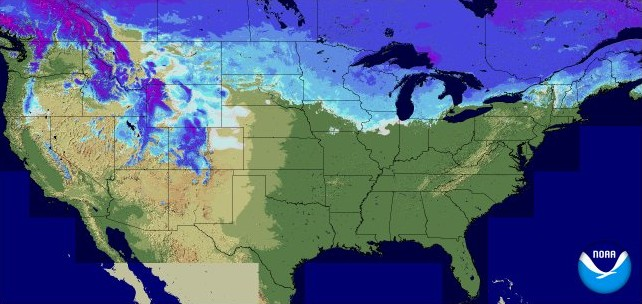
\includegraphics[width=\textwidth, trim= 0mm 0mm 0mm 0mm]{figs/snow_gt_2.jpg}
    \caption{January 15th, 2014}
    \label{fig:snow_map_2}
  \end{subfigure}
  \begin{subfigure}[b]{0.33\textwidth}
    \centering
		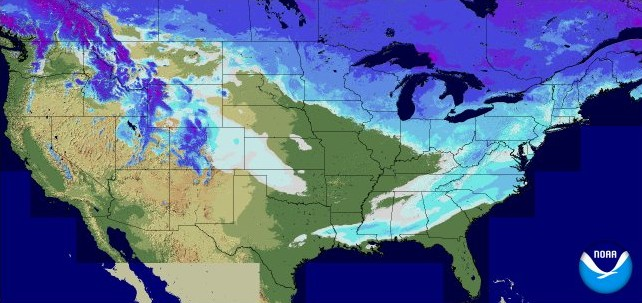
\includegraphics[width=\textwidth, trim= 0mm 0mm 0mm 0mm]{figs/snow_gt_3.jpg}
    \caption{January 29th, 2014}
    \label{fig:snow_map_3}
  \end{subfigure}
  \begin{subfigure}[b]{0.33\textwidth}
    \centering
		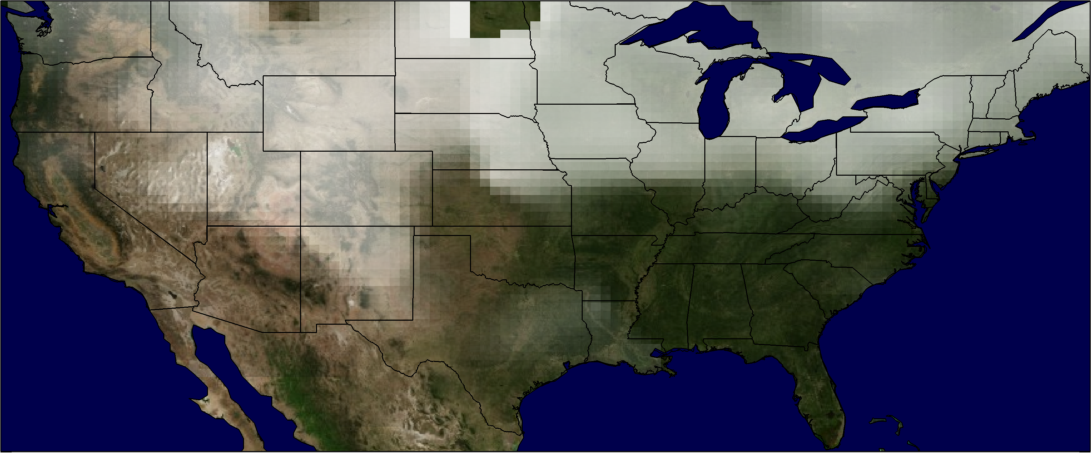
\includegraphics[width=\textwidth, trim= 0mm 0mm 0mm 0mm]{figs/snow_map_1.png}
    \caption{January 1st, 2014}
    \label{fig:snow_map_1}
  \end{subfigure}
  \begin{subfigure}[b]{0.33\textwidth}
    \centering
		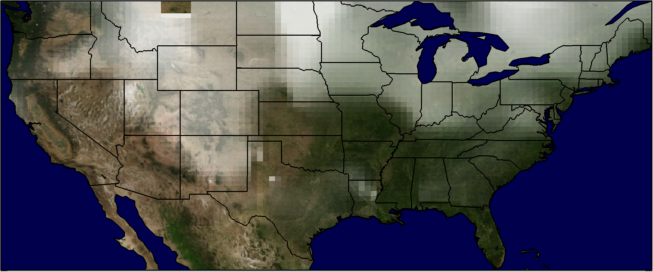
\includegraphics[width=\textwidth, trim= 0mm 0mm 0mm 0mm]{figs/snow_map_2.png}
    \caption{January 15th, 2014}
    \label{fig:snow_map_2}
  \end{subfigure}
  \begin{subfigure}[b]{0.33\textwidth}
    \centering
		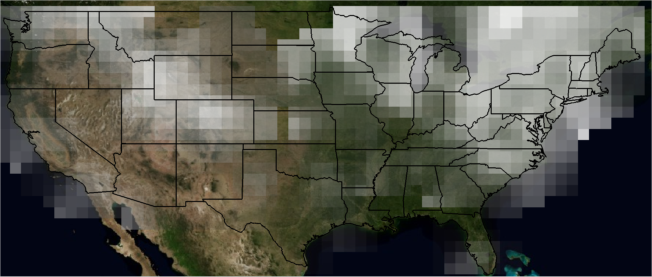
\includegraphics[width=\textwidth, trim= 0mm 0mm 0mm 0mm]{figs/snow_map_3.png}
    \caption{January 29th, 2014}
    \label{fig:snow_map_3}
  \end{subfigure}
  \caption{This shows maps of the snow attribute from webcams across the
           continental United States in the month of January, 2014 and the corresponding
           map of snow depth created using remote sensing data.\protect\footnotemark 
           The top row shows the remote sensing snow maps and the bottom row 
           shows the snow maps using the snow attribute.}
  \label{fig:snow_maps}
\end{figure*}
\footnotetext{Ground truth snow maps from: \url{http://www.nohrsc.noaa.gov/nsa/index.html}}

\begin{figure}[t]
	\centering
		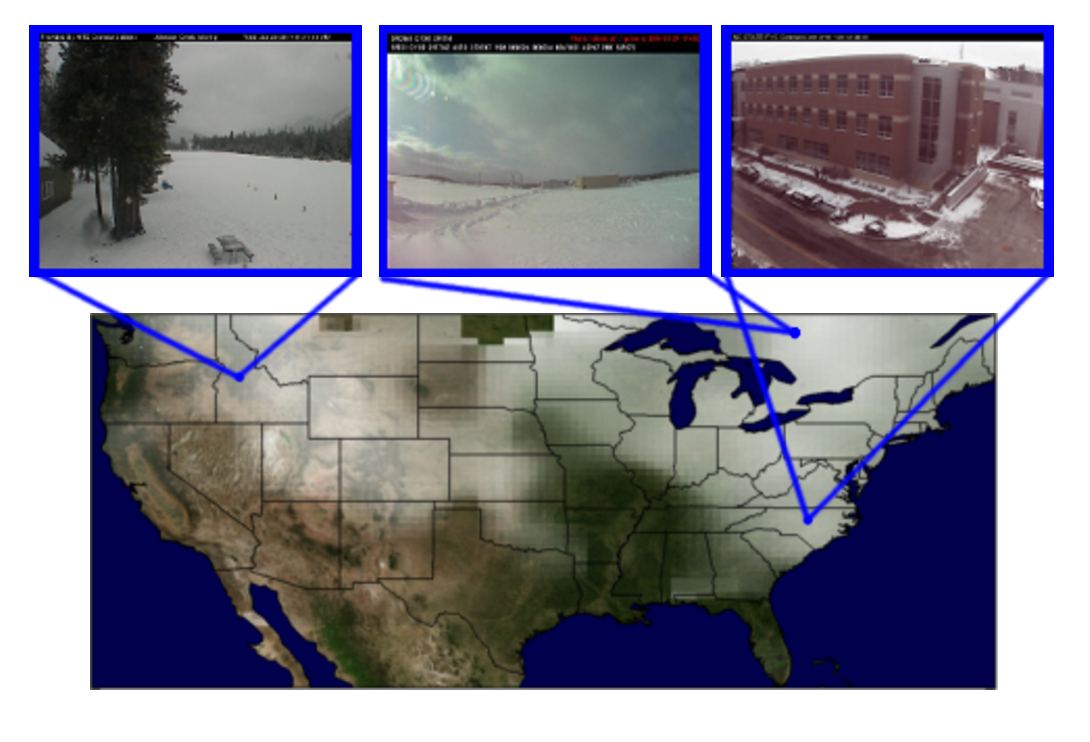
\includegraphics[width=0.5\textwidth, trim= 0mm 10mm 0mm 0mm]{figs/snow_exs.pdf}
		\caption{This shows example snowy images from collected webcam data.}
		\label{fig:snow_exs}
\end{figure}

\subsection{Weather Mapping}

We take advantage of the large number of labeled webcam images from webcams
with known locations to create maps of transient attributes across the
continental United States.  \figref{snow_maps} shows three maps for the snow
attribute across the continental United States.  Data from January 2014 for
AMOS webcams within the continental United States and the southern edge of
Canada was downloaded and labeled using TransientNet-H.  These maps show
predicted snow coverage using only transient attributes from webcam data.
Variation between the three maps shows heavy snow coverage in the beginning of
the month, snow melting in the middle of the month, and a large snow storm in
the north-east at the end of the month.  Anomalous regions of high snow values,
such as those along the California coast, likely come from webcams facing a
beach scene.  A beach with light colored sand covering the ground appears
visually similar to a snowy scene.  Several cameras of this nature were
manually pruned from the list of cameras used in \figref{snow_maps}.
\figref{snow_exs} shows example images from selected webcams on January 29th,
2014. The first two example images show heavy snow cover in northern areas, but
the third example image shows the light snow cover in the south-eastern region
of the United States.  

Maps for other attributes show expected natural phenomena (the
\textit{daylight} attribute increasing/decreasing east to west as the sun
rises/sets) and cues about the natural world (the \textit{rugged} attribute
higher in the mountainous west and low in the plains of the midwest).  Using a
method such as this one allows us to create live-updating attribute maps of an
area with webcam data.  The images are labeled as they are captured, updating
the map with the new attribute values. 

\section{Application to Webcam Geolocalization}

In this section, we show that it is possible to geolocalize webcams
using their transient attributes. Since the local weathers vary
from place to place, the changing pattern of weather attribute can be
treat as a figure print in that region.

Using the framework proposed in~\cite{jacobs07geolocate}, we replace
the webcam PCA coefficents with transient attribute features. The
geolocalization is done by computing the correlation map between pixel
density of satellite imagery and webcam transient attribute features.


\section{Conclusions}
We introduce a fast method for predicting transient scene properties in a
single image.  Deep convolutional neural networks achieve state-of-the-art
results for predicting these transient scene properties, as well as two class
weather classification.  The CNNs require no hand-engineered features, are
simple to train, are very fast at test time, and make accurate predictions. In
addition, these networks can be quickly extended to label additional attributes
or adapted to new datasets with a small amount of retraining.  The speed up
provided by the CNNs allows us to predict transient scene properties for vast
amounts of real-world data and propose several applications of the properties.
We use this to label a large collection of webcam data and create year-long
summaries for each webcam.  We also use a ``fully- convolutional'' network to
show where attributes occur within an image.

%We introduce six deep convolutional neural networks for predicting transient
%scene attributes from a single image. These networks achieve state-of-the-art
%results on two benchmark datasets. The key advantages of the proposed approach
%are that it requires no hand-engineered features, is simple to train, is very
%fast at test time, and makes accurate predictions. In addition, these networks
%can be quickly extended to label additional attributes or adapted to new datasets
%with a small amount of retraining.  We demonstrate the real world
%ability of our methods for the task of automatically labeling outdoor
%webcams.
%
%In future work, we plan to explore the use of these networks in an
%application to micro-climate estimation from publicly available
%outdoor webcams~\cite{islam13webcamweather}. 

{\small
\bibliographystyle{IEEEbib}
\bibliography{refs}
}

\end{document}
